\chapter{\label{cha:tm_sentence_encoders}Sentence Encoders for Translation Memories}
Matching and retrieving previously translated segments from a Translation Memory is the key functionality in Translation Memories (TM) systems. This matching and retrieving process is still limited to algorithms based on edit distance in most commercial TM systems. However, edit distance is unable to accurately capture the similarity between segments when different wording and syntactic structures are used to express the same idea \autocite{mitkov2008improving}. As a result, even if the TM contains a semantically similar segment, the retrieval algorithm will not identify it in most cases. In Chapter \ref{cha:tm_introduction}, we identified this as a major drawback in TMs.

Researchers address this shortcoming of the edit distance metric in so-called "third-generation" TM tools by employing similarity metrics that can identify semantically similar segments even when they are different at token level \autocite{pekar2007new}. As we stated in Part I of the thesis, deep learning based architectures are the state-of-the-art in calculating STS between texts. Furthermore, as we have shown multiple times, they can be easily adapted for different languages and domains. Therefore, having a deep learning based STS metric would benefit TMs in many ways \autocite{ranasinghe:2021}. In this chapter, we will continue the idea of "third-generation" TM tools by employing deep learning based STS metrics in TM matching and retrieving algorithms. 


As discussed in Chapter \ref{cha:sts_transformers}, the transformers have set the state-of-the-art performance on semantic textual similarity. However, to predict the similarity at test time, both sentences must be fed into the transformer network, which causes a massive computational overhead \autocite{reimers-gurevych-2019-sentence}. Finding the most similar sentence to the incoming sentence in a collection of 100,000 sentences take $\sim$1 hour with transformers. This would not be efficient enough for TMs. Therefore, we had to take a step back from Transformers and look for alternative STS solutions. 

As discussed in Part I of the thesis, the next best STS method we experimented with were Siamese architectures, explored in Chapter \ref{cha:sts_siamese_neural_networks}. The advantage of Siamese architectures is that they can also be used as sentence encoders. Therefore, they don't need to have both sentences in the network at inference time. Sentence embeddings for the sentences in the TM can be calculated in advance and stored in a database. Then, when a new sentence comes in for the TM system, the algorithm gets the embeddings for that sentence and performs a simple similarity measure across the sentence embeddings in the TM to find a match. This process require less time compared to transformers. Therefore, we utilised the best Siamese architecture we had in Part I of the thesis; Sentence-BERT \autocite{reimers-gurevych-2019-sentence} in the TM experiments we perform in this Chapter. In order to have a diverse set of algorithms, we also used the best sentence encoders we had in Chapter \ref{cha:sts_sentence_encoders}; Infersent \autocite{conneau-EtAl:2017:EMNLP2017} and Universal Sentence Encoder \autocite{cer2018universal}. As far as we know, this is the first study to employ deep learning in TM systems. 

We address two research questions in this chapter:

\textbf{RQ1}: Are the sentence encoders efficient enough for TM matching and retrieval tasks?

\textbf{RQ2}: How do the sentence encoders perform in TM retrieving task compared to other TM tools?

The main contributions of this chapter are as follows.

\begin{enumerate}
	\item We evaluate three sentence encoders in the TM retrieval task in English-Spanish segments using a real-world TM; DGT-TM. We compare the results against a popular TM system; Okapi\footnote{The Okapi Framework is a cross-platform and free open-source set of components and applications that offer extensive support for localising and translating documentation and software. It is available on \url{https://okapiframework.org/}. We specifically use the Rainbow application available in the framework, which allows bulk matching and retrieval from a translation memory.}; which uses edit distance for the retrieval process.
	
	\item Evaluations are carried out separately for different fuzzy match ranges, and we show that sentence encoders outperform Okapi in certain fuzzy match ranges.
	
	\item We further perform a detailed human evaluation of the matches retrieved from sentence encoders and Okapi, collaborating with three native Spanish speakers with a translation background. We show that sentence encoders generally provide better matches than Okapi.
	
	\item The code used for the experiments conducted are publicly available to the community\footnote{The public GitHub repository is available on \url{https://github.com/tharindudr/intelligent-translation-memories}}.
\end{enumerate}

The rest of this chapter is organised as follows. Section \ref{sec:tm_sentence_encoders_motivation} describes our motivation for the study comparing the performance of edit distance against sentence encoders in STS tasks. In section \ref{sec:tm_sentence_encoders_method}, we present the methodology we used to incorporate sentence encoders in to TM systems. Section \ref{sec:tm_sentence_encoders_results} presents the results we got with sentence encoders for English-Spanish sentence pairs in DGT-TM. In section \ref{sec:tm_sentence_encoders_error}, we provide a detailed human evaluation done by three native Spanish speakers identifying the strengths and weaknesses of the proposed approach. The chapter finishes with conclusions and ideas for future research directions in TM matching and retrieving.


\section{Motivation}
\label{sec:tm_sentence_encoders_motivation}
We first evaluated the edit distance in two of the STS datasets introduced in Chapter \ref{cha:sts_introduction}; SICK and STS 2017. We compared these results to the results we got from sentence encoders in Chapter \ref{cha:sts_sentence_encoders}. Considering the accuracy of the STS task, we used Infersent2 from the pre-trained Infersent models, transformer encoder from the pre-trained Universal Sentence Encoder models and stsb-roberta-base-v2 from the pre-trained SBERT models which is based on RoBERTa \autocite{liu2019roberta}. 

With the SICK dataset, edit distance only achieved 0.361 Pearson correlation while Infersent, Universal Sentence Encoder and SBERT achieve 0.769, 0.780 and 0.892 Pearson correlation, respectively. Similarly, with the STS 2017 dataset, sentence encoders outperform edit distance by a large margin. This is a clear indication that the sentence encoders can calculate text similarity better than edit distance. To further confirm this, we analysed the results of individual sentence pairs. Table \ref{tab:sts_evaluation} shows some of the example sentence pairs from STS2017, where sentence encoders showed promising results against edit distance.  

\begin{table}[t] 
	\centering
	\scalebox{0.73}{
	\begin{tabular}{ |p{4.5cm}|p{4.5cm}|c|c|c|c|c| }
		\hline
		\multicolumn{1}{|c|}{\textbf{Sentence 1}} & \multicolumn{1}{c|}{\textbf{Sentence 2}} &  \textbf{GOLD} & \textbf{ED} & \textbf{Infersent} & \textbf{USE} & \textbf{SBERT} \\
		\hline
		Israel expands subsidies to settlements & Israel widens settlement subsidies & 1.0000 & 0.0214 & 0.8524 & 0.8431 & 0.8997\\
		\hline
		A man plays the guitar and sings. & A man is singing and playing a guitar. & 1.0000 & 0.0124 & 0.7143 & 0.7006 & 0.8142 \\
		\hline
		A man with no shirt is holding a football & A football is being held by a man with no shirt & 1.0000 & 0.0037 & 0.9002 & 0.8852 & 0.9267\\
		\hline
		EU ministers were invited to the conference but canceled because the union is closing talks on agricultural reform, said Gerry Kiely, a EU agriculture representative in Washington. & Gerry Kiely, a EU agriculture representative in Washington, said EU ministers were invited but canceled because the union is closing talks on agricultural reform. & 1.0000 & 0.1513 & 0.7589 & 0.7865 & 0.8190\\
		\hline
		
	\end{tabular}
	}
	\caption[Examples sentence pairs where sentence encoders performed better than edit distance in the STS task.]{Examples sentence pairs where sentence encoders performed better than edit distance in the STS task. The \textbf{GOLD} column shows the score assigned by humans, normalised between 0 and 1. The \textbf{ED} column shows the similarity obtained regarding the edit distance. \textbf{Infersent}, \textbf{USE} and \textbf{SBERT} columns show the similarity obtained by Infersent, Universal Sentence Encoder and SBERT respectively. 
	}
	\label{tab:sts_evaluation}
\end{table}

As can be seen in Table \ref{tab:sts_evaluation}, all of the sentence encoders handle semantic textual similarity better than edit distance in many of the cases where the word order is changed in two sentences, but the meaning remains the same. The detection of similarity, even when the word order is changed, will be important in segment matching and retrieval in TMs, which is the motivation for this study.


\section{Methodology}
\label{sec:tm_sentence_encoders_method}

We conducted the following steps for all three sentence encoders mentioned before; Infersent, Universal Sentence Encoder and SBERT. We used the same pre-trained models mentioned in Section \ref{sec:tm_sentence_encoders_motivation}. As discussed in Chapter \ref{cha:tm_introduction}, for all the experiments, we used DGT-TM 2018 Volume 1 as the translation memory and 2018 Volume 3 - as the source for input sentences. 


	\paragraph{Step 1}: Calculated the sentence embeddings for each segment in the translation memory (230,000 segments) and stored the vectors in AquilaDB\footnote{AquilaDB is available on \url{https://github.com/Aquila-Network/AquilaDB}}. AquilaDB is a decentralised vector database used to store feature vectors and perform k-nearest neighbours (KNN) retrieval. It is built on top of the popular Apache CouchDB\footnote{CouchDB is available on \url{https://github.com/apache/couchdb}}. A record of the database has three fields: source segment, target segment and the source segment vector.
	
	\paragraph{Step 2}: Calculated the sentence embedding for one incoming segment. 
	
	\paragraph{Step 3}: Calculated the cosine similarity of that embedding with each of the embedding in the database. We retrieve the embedding with the highest cosine similarity and retrieve the corresponding target segment for the embedding as the translation memory match. We used the \textit{'getNearest'} functionality provided by AquilaDB for this step. This step is visualised in Figure \ref{fig:TM}.
	
	
	
	
	\begin{figure}[ht]
		\centering
		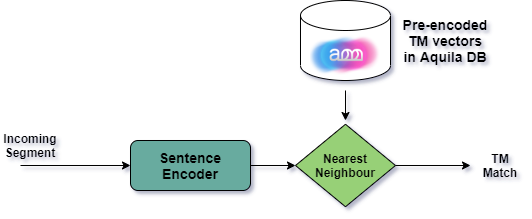
\includegraphics[scale=0.6]{figures/translation_memories/sentence_encoders/TM.png}
		\caption[TM Matching Process for an Incoming Segment]{TM matching process for an incoming segment.}
		\label{fig:TM}
	\end{figure}
	

The efficiency of the TM matching and retrieval is a key factor for the translators using them. As discussed in Chapter \ref{cha:tm_introduction}, most of the proposed third-generation TM systems were not fast enough to be used in real-world scenarios. This is also the reason why they are not popular in the community. We wanted to avoid making the same mistake with our proposed approach to make it more useful for the community. Therefore, as the first step, we calculated the efficiency of the proposed method. 

Table \ref{tab:tm_efficiency}, discusses the efficiency of each sentence encoder. The experiments were done in an Intel(R) Core (TM) computer with i7-8700  CPU and 3.20GHz clock speed. While the performance of the sentence encoders would be more efficient in a GPU (Graphics Processing Unit), we carried our experiments in a CPU (Central Processing Unit) since the translators using translation memory tools are unlikely to have access to a GPU on a daily basis. 


\begin{table}[t]
	\centering
		\begin{tabular}{|c|c|c|c|}
			\hline
			\textbf{Architecture} & \textbf{Step 1} & \textbf{Step 2} & \textbf{Step 3}\\ 
			\hline
			USE & 108s & 1.23s & 0.40s \\
			Infersent & 496s & 0.022s & 0.40s \\
			SBERT & 1102s & 0.052s & 0.52s \\
			\hline
		\end{tabular}
		\caption[Time for each step with experimented sentence encoders.]{Time for each step with experimented sentence encoders.}
		\label{tab:tm_efficiency}
\end{table}

The translation memory was processed in batches of 256 sentences to obtain sentence embeddings. As seen in Table \ref{tab:tm_efficiency}, the Universal Sentence Encoder(USE) was the most efficient encoder, delivering sentence embeddings within 108 seconds for 230,000 sentences. At the other end of the scale was Sentence-BERT, which took 1102 seconds to derive the sentence embeddings for the same number of sentences in the translation memory. Even though these times may appear very long, we should keep in mind that this process needs to be done only once as they are kept in a database and do not need to be computed again. 

The second column of Table \ref{tab:tm_efficiency} reports the time needed for each sentence encoder to embed a single sentence. Input sentences were not processed in batches as was done for the TM sentences. The rationale behind this decision is the fact that the translators translate sentences one by one. Interestingly, while the Universal Sentence Encoder was the most efficient in generating sentence embeddings in batches, it was the least efficient encoder to derive the embedding for a single sentence where it took 1.23 seconds to do so. InferSent was the fastest sentence encoder for a single sentence. 

The third column of Table \ref{tab:tm_efficiency} reports the time needed to retrieve the best match from the translation memory. This includes the time taken to compute the cosine similarity between the embeddings of TM sentences and the embeddings of the input sentence. It also consists of the time to sort the similarities, get the index of the highest similarity, and retrieve the TM sentence considered a match for the input sentence. As shown in Table \ref{tab:tm_efficiency}, all sentence encoders needed approximately 0.5 seconds to perform this operation. As a whole, to identify the best match from the translation memory, InferSent and Sentence-BERT encoders did not take more than 1 second, while Universal sentence encoder took 1.6 seconds which is considered good enough for an operational translation memory tool. 

With these observations, we answer our \textbf{RQ1}: sentence encoders are efficient enough for TM matching and retrieval tasks. The numbers we calculated for each step provide evidence that the proposed methods are fast enough to be used in a real-world environment and represent a huge improvement over the existing third-generation TM systems in terms of efficiency.


\section{Results and Evaluation}
\label{sec:tm_sentence_encoders_results}
In this section, we report the results of the three selected sentence encoders in TM matching. We ran automatic evaluation experiments by comparing the matches returned by Okapi, which uses a simple variant of edit distance as the retrieving algorithm and the matches returned by each of the sentence encoders. To measure the quality of a retrieved segment, the METEOR score was computed between the translation of the incoming sentence, as present in the DGT-TM 2018, and the translation of the match retrieved from the translation memory. This process was repeated for the segments retrieved by our deep learning methods and those retrieved using Okapi. 

\begin{table}[ht!]
	\centering
		\begin{tabular}{|c|c|c|c|c|c|}
			\hline
			\textbf{Fuzzy score} & \textbf{Okapi} & \textbf{USE} & \textbf{Infersent} & \textbf{SBERT} & \textbf{Amount} \\ 
			\hline
			0.8-1.0 & \textbf{0.931} & 0.854 & 0.864 & 0.843 &1624\\
			\hline
			0.6-0.8 & 0.693 & 0.702 & \textbf{0.743} & 0.698 & 4521\\
			\hline
			0.4-0.6 & 0.488 & 0.594 & \textbf{0.630} & 0.602 & 6712\\
			\hline
			0.2-0.4 & 0.225 & 0.318 & \textbf{0.347} & 0.316 & 13136 \\
			\hline
			0-0.2 & 0.011 & 0.128 & \textbf{0.134} & 0.115 & 24612 \\
			\hline
		\end{tabular}
		\caption[Result comparison between Okapi and the sentence encoders]{Result comparison between Okapi and the sentence encoders for each partition. The \textbf{Fuzzy score} column represents the each partition. The \textbf{Okapi} column shows the average METEOR score between the matches provided by the Okapi and the actual translations in that partition. The \textbf{USE}, \textbf{Infersent} and \textbf{SBERT} columns show the average METEOR score between the matches provided by each of the sentence encoders and the actual translations in that partition. The \textbf{Amount} column shows the number of sentences in each partition. The best result for each partition is shown in bold.}
		\label{tab:tm_sentence_encoder_results}
\end{table}

For a better comparison, we first removed the sentences where the matches provided by Okapi and the sentence encoders were the same. Next, in order to analyse the results, we divided the results into five partitions according to the fuzzy match score retrieved from Okapi: 0.8 –- 1, 0.6 –- 0.8, 0.4 –- 0.6, 0.2 –- 0.4, and 0 –- 0.2. These ranges were selected to understand the behaviour of the sentence encoders in the TM matching and retrieval task. The first partition contained the matches derived from Okapi with a fuzzy match score between 0.8 and 1. We calculated the average METEOR score for the segments retrieved from Okapi and for the segments retrieved from each of the sentence encoders in this particular partition. We repeated this process for all of the partitions. Table \ref{tab:tm_sentence_encoder_results} lists the results for each sentence encoder and Okapi. 

As can be seen in Table \ref{tab:tm_sentence_encoder_results}, for the fuzzy match score range 0.8-1.0, the Okapi METEOR score mean is higher than any of the mean METEOR scores of the sentence encoders which indicates that the matches returned in that particular fuzzy match score range, by Okapi, are better than the matches returned by any of the sentence encoders. However, in the rest of the fuzzy match score ranges, the sentence encoders outperform Okapi, which shows that for the fuzzy match score ranges below 0.8, the sentence encoders offer better matches than Okapi. From the sentence encoders, InferSent performs better than both the Universal Sentence Encoder and SBERT. The results in Table \ref{tab:tm_sentence_encoder_results} show that when there are close matches in the Translation Memory, edit distance delivers better matches than the sentence encoders. However, when the edit distance fails to find a proper match in the TM, the match offered by the sentence encoders will be better. 

Usually, the TM matches with lower fuzzy match scores (< 0.8) are not used by professional translators, or when used, they lead to a decrease in translation productivity. But our method can provide better matches to sentences below fuzzy match score 0.8, hence improving the translator's productivity. According to the annotation guidelines of STS tasks which we explained in Chapter \ref{cha:sts_introduction}, an STS score of 0.8 means \textit{"The two sentences are mostly equivalent, but some unimportant details differ"} and an STS score of 0.6 means \textit{"The two sentences are roughly equivalent, but some important information differs/missing"}. If we further analyse the fuzzy match score range 0.6-0.8, as shown in table \ref{tab:tm_sentence_encoder_results}, the mean semantic textual similarity for the sentences provided by Infersent is 0.743. Therefore, we can assume that the matches retrieved from Infersent in the fuzzy match score range 0.6-0.8 will help to improve the translation productivity.


With these observations, we answer our \textbf{RQ2}: sentence encoders can improve TM matching and retrieval, especially in the lower fuzzy match scenarios. The proposed process would improve the current third-generation TM tools as it provides good results and is very efficient.

\section{Error Analysis}
\label{sec:tm_sentence_encoders_error}
As mentioned in Chapter \ref{cha:tm_introduction}, automatic machine translation evaluation metrics such as METEOR are far from perfect. As METEOR relies largely on string overlap, it cannot properly capture the semantic equivalence of the segments retrieved using the sentence encoders. Therefore, a human evaluation is required for this study. In this section, we carried out a human evaluation in the form of error analysis.

Three native Spanish speakers with backgrounds in translation went through the matches provided by the sentence encoders and the matches provided by Okapi. The usual pattern they found was that the sentence encoders returned better results; however, there were a limited number of cases where Okapi performed better. The native speakers analysed more than one thousand segments, and below is a brief analysis of the typical error cases they found.

In a number of cases, InferSent performed better than Okapi because the latter proposed translations that contained information that did not appear in the English input segment. As an illustration of this typical case, for the input segment (1) for which the correct translation is (2) Okapi retrieved (3) whilst InferSent selected (4), which is more appropriate. 

\begin{enumerate}[label={(\arabic*)}]
	\item The audit shall include.
	\item La evaluación incluirá.
	\item Los indicadores de rendimiento incluirán. (Key performer indicators shall include)
	\item El informe incluirá. (The report shall include)
\end{enumerate}

In other cases, Okapi selects segments that capture only a part of the meaning of the input segment correctly but fails to provide its whole meaning. For example, for the input segment (5), Okapi selects (6). Due to its exclusive reliance on edit distance, Okapi selects a segment that has the correct temporal expression (16 June/16 de junio), but the rest of the retrieved translation does not have any connection with the original. In contrast, InferSent can retrieve a segment that conveys the meaning correctly but has the incorrect date (7). From the point of view of the effort required to produce an accurate translation, the segment selected by InferSent requires less effort (as the translator only need to correct the date ) than the one selected by Okapi. 

\begin{enumerate}[resume,label={(\arabic*)}]
	\item It shall apply in all Member States from 16 June 2020.
	\item A partir del 16 de junio de 2024, los Estados miembros utilizarán la función de registro centralizada. (Member States will use the centralised registration function from 16 June 2024)
	\item Los Estados miembros aplicarán dichas disposiciones a partir del 21 de diciembre de 2020. (These provisions shall apply in all Member States from 21 December 2020)
	
\end{enumerate}

The advantage of sentence encoders can also be observed when comparing the performance of Okapi with the Universal Sentence Encoder. Okapi often recognises only a part of the English sentences. Therefore, the match suggested is only partially correct. As an illustration, for segment (8), Okapi retrieved (9) as a match. The word brief does not appear in the retrieved text, and additionally, Okapi adds "de las mercancías". The translation retrieved by the Universal Sentence Encoder (10) is correct. This pattern can also be seen when comparing Okapi with SBERT. For example, while the proposed match for (11) by SBERT is correct (12), Okapi only recognises one word of the segment, as the retrieved match is (13). 

\begin{enumerate}[resume,label={(\arabic*)}]
	\item	Brief description
	\item	Descripción de las mercancías (Goods description)
	\item	Breve descripción
	\item	Test equipment
	\item	Los equipos de ensayo (The test equipment)
	\item	Equipo informático (IT equipment)
\end{enumerate}


In general, and on a number of occasions, Okapi omits some of the information that the sentence encoders identify. The equivalent of the sentence (14) is retrieved by Okapi as (15), with edible offal missing in Okapi’s proposal. The sentence retrieved from InferSent, however conveys this information (16).

\begin{enumerate}[resume,label={(\arabic*)}]
	\item	Edible offal of bovine animals, frozen
	\item	De la especial bovina, congelados (Bovine animals, frozen)
	\item	Carne de animales de la especie bovina, congelada. (Meat of bovine animals, frozen.)
\end{enumerate}

Okapi often fails not only with whole sentences but also with segments that only contain one word. When retrieving the translation of the word (17), the sentence encoder InferSent suggest (18), whereas Okapi also adds the word Lugar (19). This also happens with (20), which InferSent returns as (21), whereas Okapi retrieves (22); the word elección (choice) does not appear in the English sentence. In addition, Okapi often fails with multiword expressions. Okapi retrieves the translation of the multiword expression (23) as (24), and in this case, the proposed match features redundant information. The segment retrieved by SBERT represents the best solution (25).

\begin{enumerate}[resume,label={(\arabic*)}]
		\item	Date
		\item	Fecha
		\item	Lugar y fecha (Place and date)
		\item	Fuel
		\item	Combustible
		\item	elección del combustible (choice of fuel)
		\item	Engine type
		\item	Potencia del motor principal en KW: Marca: Tipo (Main engine power in KW: Make: Type)
		\item	Tipo de motor
	
\end{enumerate}

There are cases where the segment retrieved from the sentence encoder is similar to the one retrieved from Okapi, but the sentence encoder is better at conveying subtle nuances. For instance, the proposed translation for sentence (26) by Okapi is (27), and the sentence retrieved from the Universal Sentence Encoder is (28). The nuance refers to the proposed translation for as appropriate. Okapi returns (29), whereas the Universal Sentence Encoder retrieves the correct translation (30). Another similar example where Okapi fails is the retrieved translation of (31) as (32); the Universal Sentence Encoder acts correctly on this occasion.

\begin{enumerate}[resume,label={(\arabic*)}]
	\item	This Decision shall be kept under constant review and shall be renewed or amended, as appropriate, if the Council deems that its objectives have not been met.
	\item	Se prorrogará o modificará, si procede, en caso de que el Consejo estime que no se han cumplido los objetivos de la misma. (This Decision shall be renewed or amended, if appropriate, if the Council deems that its objectives have not been met)
	\item	Será prorrogada o modificada, según proceda, si el Consejo considera que no se han cumplido sus objetivos. (This Decision shall be renewed or amended, as appropriate, if the Council deems that its objectives have not been met)
	\item	si procede (if appropriate)
	\item	según proceda (as appropriate)
	\item	if applicable
	\item	no procede (not applicable)
\end{enumerate}

There are several cases where Okapi returns a completely incorrect translation as opposed to the sentence encoders. For (33), Okapi proposed (34), which has nothing to do with the original meaning. The Universal Sentence Encoder offers a simple yet good solution (35). 

\begin{enumerate}[resume,label={(\arabic*)}]
	\item	None of the above
	\item	Veánse los considerandos 92 a 94 (See items 92 to 94)
	\item	Ninguna (None)
	
\end{enumerate}

There are a limited number of cases where Okapi fares better than the sentence encoders. One such example is when encoders retrieve matches of named entities. By way of illustration, the translation the Universal Encoder retrieves for (36) is (37) instead of (38); SBERT retrieves (39) when the original segment is (40), and the proposal by InferSent for (41) is (42). 

\begin{enumerate}[resume,label={(\arabic*)}]
	\item	Japan
	\item	Israel
	\item	Japón
	\item	Singapur (Singapore)
	\item	Philippines
	\item	within municipality of Sitovo
	\item	en el municipio de Alfatar (within municipality of Alfatar)
\end{enumerate}

Finally, and occasionally, sentence encoders could also propose translations featuring redundant information which does not appear in the original English segment. The match InferSent returns for (43) is (44), and in this case, Okapi retrieves a correct translation (45). On another isolated occasion, SBERT also adds a redundant word "mixto" (joint) by proposing (46) as the translation for (47). In this particular instance, the retrieved match by Okapi is correct (48). 

\begin{enumerate}[resume,label={(\arabic*)}]
\item	Requirements
\item	Requisitos del Eurosistema (Eurosystem requirements)
\item	Requisitos
\item	El Comité mixto adoptará su reglamento interno (The joint Committee shall establish its own rules of procedures)
\item	The Committee shall establish its own rules of procedures
\item	El Comité dispondrá su reglamento interno
\end{enumerate}

This analysis also clearly indicates that sentence encoders provide better matches than Okapi in most scenarios. It further confirms our answer to \textbf{RQ2} that sentence encoders can be used to improve the matching and retrieval process in TMs.

\section{Conclusions}
Third-generation TM tools have addressed the limitations of traditional TM tools. Yet, they are not popular in the community since they are largely inefficient, and there is not much performance gain from using them. To address this, we propose to use the deep learning based STS metrics that we experimented with in Part I of the thesis in TMs. Considering both accuracy and efficiency, we picked three sentence encoders; Infersent, Universal Sentence Encoder and SBERT and designed a TM matching algorithm based on them. We evaluated the proposed algorithm in a real-world TM; DGT-TM. We compared the results from each of the sentence encoders with the results from Okapi, which uses edit distance to acquire the best match from the translation memory.  The results show that the sentence encoders return better matches than simple edit distance for sentences with a fuzzy match score less than 0.8 in Okapi. Of the sentence encoders, InferSent fares best. We also present an error analysis, where three native Spanish speakers analysed the matches proposed by the sentence encoders and Okapi. This error analysis further confirms that the sentence encoders can be used to improve the matching and retrieval process in TMs \autocite{ranasinghe-etal-2020-intelligent}. 

The main limitation of the proposed algorithm is the time taken to retrieve a match can be high with a large TM. This is a common problem for deep learning applications, which is usually solved by employing GPUs. However, in this case, it would not be feasible to use GPUs since they are expensive, and translators using translation memory tools would not have access to GPUs on a daily basis. To overcome this impediment, we envisage the deployment of algorithms to filter out the sentences from the TM before the retrieval process and make the cosine similarity calculation between vectors a computationally less intensive process. Faster algorithms generating sentence embeddings such as averaging word embeddings, which we discussed in Chapter \ref{cha:sts_state_of_the_art_methods}, will be used in these experiments. 

The automatic evaluation metric that we used in this study, METEOR, has its limitations that might have affected the evaluation of this study. Very recently, new automatic MT evaluation metrics such as BLEURT \autocite{sellam-etal-2020-bleurt} which are based on transformers, have been proposed. Unlike METEOR, these metrics do not rely greatly on string overlap and would be more suitable for this study. Therefore, as future work, we will incorporate these new automatic MT evaluation metrics.

With this, we conclude Part II of the thesis, using deep learning based STS metrics in translation memories. We showed that the STS methods we experimented with in Part I of the thesis can be successfully employed in TMs. Our methods outperform edit distance based TM matching and retrieval algorithms. Furthermore, the proposed method is very efficient and can be used in real-world scenarios. Therefore, we believe that the findings of Part II of the thesis pave a new direction for third-generation TM systems.

 

